%Copyright 2014 Jean-Philippe Eisenbarth
%This program is free software: you can
%redistribute it and/or modify it under the terms of the GNU General Public
%License as published by the Free Software Foundation, either version 3 of the
%License, or (at your option) any later version.
%This program is distributed in the hope that it will be useful,but WITHOUT ANY
%WARRANTY; without even the implied warranty of MERCHANTABILITY or FITNESS FOR A
%PARTICULAR PURPOSE. See the GNU General Public License for more details.
%You should have received a copy of the GNU General Public License along with
%this program.  If not, see <http://www.gnu.org/licenses/>.

%Based on the code of Yiannis Lazarides
%http://tex.stackexchange.com/questions/42602/software-requirements-specification-with-latex
%http://tex.stackexchange.com/users/963/yiannis-lazarides
%Also based on the template of Karl E. Wiegers
%http://www.se.rit.edu/~emad/teaching/slides/srs_template_sep14.pdf
%http://karlwiegers.com
\documentclass{scrreprt}
\usepackage{listings}
\usepackage{underscore}
\usepackage{graphicx}
\usepackage{svg}
\usepackage[bookmarks=true]{hyperref}
\usepackage[utf8]{inputenc}
\usepackage[english]{babel}
\usepackage{hyperref}
\hypersetup{
    bookmarks=false,    % show bookmarks bar?
    pdftitle={Software Requirement Specification},    % title
    pdfauthor={VER VALEM Willian BAYOL Elmer LOPEZ-FARFAN M. Liliana TAGNAOUTI Khaoula},                     % author
    pdfsubject={TeX and LaTeX},                        % subject of the document
    pdfkeywords={TeX, LaTeX, graphics, images}, % list of keywords
    colorlinks=true,       % false: boxed links; true: colored links
    linkcolor=blue,       % color of internal links
    citecolor=black,       % color of links to bibliography
    filecolor=black,        % color of file links
    urlcolor=purple,        % color of external links
    linktoc=page            % only page is linked
}%
\def\myversion{1.0 }
\date{}
%\title
\usepackage{hyperref}
\begin{document}

\begin{flushright}
    \rule{16cm}{5pt}\vskip1cm
    \begin{bfseries}
        \Huge{SOFTWARE REQUIREMENTS\\ SPECIFICATION}\\
        \vspace{1.9cm}
        for\\
        \vspace{1.9cm}
        Dominion Logs Datamining\\
        \vspace{1.9cm}
        Prepared by \\ VER VALEM Willian \\ BAYOL Elmer \\ LOPEZ-FARFAN M. Liliana
        \\ TAGNAOUTI Khaoula\\
        \vspace{1.9cm}
        \today\\
    \end{bfseries}
\end{flushright}

\tableofcontents


% \chapter*{Revision History}

% \begin{center}
%     \begin{tabular}{|c|c|c|c|}
%         \hline
%       Name & Date & Reason For Changes & Version\\
%         \hline
%       21 & 22 & 23 & 24\\
%         \hline
%       31 & 32 & 33 & 34\\
%         \hline
%     \end{tabular}
% \end{center}

\chapter{Introduction}

\section{Purpose}
%But
% Identify the product whose software requirements are specified in this
% document, including the revision or release number. Describe the scope of the
% product that is covered by this SRS, particularly if this SRS describes only
% part of the system or a single subsystem.
This Document has as purpose to clarify and describe as precisely as possible the
requirements for the development of the program \textit{Dominion DataMining}.\\
\textit{Dominion DataMining} is a program which consists of 3 parts:
%Ce document a pour but de clarifier et de décrire aussi précisément que possible les besoins pour le développement du programme « Dominion DataMining ».
%Dominion DataMining est un programme qui se compose de 3 parties:*/

\begin{itemize}
  \item \textbf{Data modeling} \- Responsible to read and remodel the data to be stored.
  \item \textbf{Data Storage} \- Store the parsed data
  \item \textbf{Data analyzer} \- Responsible to query the database and generate
    human readable statistics and plot charts.
%Modélisation des données: Responsable à lire et à remodeler les données à stocker.
%Stockage de données: Conserver les données analysées.
%Analyseur de données: Responsable pour interroger la base de données et de générer des statistiques lisibles par l'homme et des graphiques de tracé.
\end{itemize}

%This requirements Specification is based on the version 0.0.1 of the program.



 \section{Intended Audience and Reading Suggestions}
%Public visé et suggestions de lecturePublic visé et suggestions de lecture
% Describe the different types of reader that the document is intended for,
% such as developers, project managers, marketing staff, users, testers, and
% documentation writers. Describe what the rest of this SRS contains and how it is
% organized. Suggest a sequence for reading the document, beginning with the
% overview sections and proceeding through the sections that are most pertinent to
% each reader type.
This document is intended for any individual user ,developer, tester, project manager or
documentation writer that needs to understand the basic system architecture and its specifications.\\
Here are the potential uses for each one of the reader types:\\
\begin{itemize}
%Ce document est destiné à tout utilisateur, développeur, testeur, chef de projet ou de la documentation écrivain qui a besoin de comprendre l'architecture de base du système et de ses spécifications.
%Voici les utilisations potentielles pour chacun des types de lecteurs:
\item \textbf{Developer: }The developer who wants to read, change, modify or add new requirements into
the existing program, must firstly consult this document and update the requirements with
appropriate manner so as to not destroy the actual meaning of them and pass the information
correctly to the next phases of the development process.\\
%Développeur: Le développeur qui veut lire, changer, modifier ou ajouter de nouveaux besoins dans le programme existant, doit tout d'abord consulter ce document et mettre à jour les besoins en manière appropriée afin de ne pas détruire leur signification réelle et de transmettre les informations correctement aux prochaines phases du processus de développement.
\item \textbf{User: }The user of this program reviews the diagrams and the specifications presented in this
document and determines if the software has all the suitable requirements and if the software
developer has implemented all of them.\\
%Utilisateur: L'utilisateur de ce programme en revue les schémas et les spécifications présentées dans ce document et détermine si le logiciel a toutes les besoins appropriés et si le développeur du logiciel a mis en œuvre tous.
\item \textbf{Tester: }The tester needs this document to validate that the initial requirements of this
program actually corresponds to the executable program correctly.\\
%Testeur: Le testeur a besoin de ce document pour vérifier que les besoins initiaux de ce programme correspondent actuellement  au programme exécutable correctement.
\end{itemize}

\section{Project Scope}
%Contexte du projet
% Provide a short description of the software being specified and its purpose,
% including relevant benefits, objectives, and goals. Relate the software to
% corporate goals or business strategies. If a separate vision and scope document
% is available, refer to it rather than duplicating its contents here.
  The \textit{Dominion} card game has been running on a server from October 2010 to March 2013. The games played on this server have been recorded in \textit{logs} that keep track of every players actions; Those \textit{logs} have been made available to the public. But some information relative to decisions made by the players haven't been recorded.
  \newline A wiki about the game has been created, it offers expert advice in decision making during the game: it mainly offers advice on a strategy level. The goal of this project, submitted by Yvan Le Borgne, researcher at the Labri, is to process the \textit{logs} (more than 12 million games) in order to answer several questions. It mainly consists in comparing the gathered data to the wiki's information in order to validate the usefulness of the ideas and informations given by experts. We will at least create validation tools offering enough efficiency.
  In order to fulfill this objective, the project's goal is to create a database containing all the games played and the to produce an analysis based on this information.
  To do so, our program will first have to extract the \textit{log} data because they are too voluminous and too complicated to use directly (non-standardized structure). We will have to set up data structures allowing us to have a better data storage. A simple way to represent this data will be offered to the user.
  Some information is also missing in the \textit{logs}(for example: cards drawn during a turn). We will try to find a method to rebuild this information and to add it to the existing information.
  We will also try to optimize the opeations made by the data analyzing by finding a balance between memorizing requests and re-computing.
  Finally, we will have to decide wich strategy is used with each game, or even recognize strategy changes during a game. We could also recognize ho applied a strategy first (who \textit{inveted} it).
  If we can detect enough strategy related data, we can also detect the usual learning process of the players.

%Le jeu de cartes Dominion a été exécuté sur un serveur à partir d'Octobre 2010 au Mars 2013. Les parties jouées sur ce serveur ont été enregistrés dans les journaux qui gardent la trace de toutes les actions des joueurs; Ces journaux ont été mis à la disposition du public. Mais certaines informations par rapport aux décisions prises par les joueurs n’ont pas été enregistrées.
%Un wiki sur le jeu a été créé, il offre des conseils d'experts dans la prise de décision au cours du jeu: il offre principalement des conseils au niveau de la stratégie. Le but de ce projet, présenté par Yvan Le Borgne, chercheur au Labri, est de traiter les journaux (plus de 12 millions de jeux) afin de répondre à plusieurs questions. Il consiste principalement à comparer les données recueillies à l'information du wiki afin de valider l'utilité des idées et des informations données par des experts. Nous allons au moins créer des outils de validation offrant suffisamment d'efficacité.
%Afin d'Atteindre cet objectif, le but du projet est de créer une base de données contenant tous les jeux joués et de produire une analyse basée sur ces informations. Pour ce faire, notre programme devra d'abord extraire les données du journal, car ils sont trop volumineux et trop compliqué à utiliser directement (structure non-standard).
%Nous aurons à mettre en place des structures de données qui nous permettent d'avoir un meilleur stockage de données. Un moyen simple pour représenter ces données sera offert à l'utilisateur.
%Certaines informations sont également manquantes dans les journaux (par exemple: les cartes tirées au cours d'un tour).
%Nous allons essayer de trouver une méthode pour reconstruire cette information et l'ajouter à l'information existante. Nous allons également essayer d'optimiser les opérations effectuées par l'analyse de données en trouvant un équilibre entre la mémorisation des demandes et le recalcule.
%Enfin, nous devrons décider quelle stratégie est utilisée avec chaque jeu, ou même reconnaître les changements de stratégie lors d'un match. Nous pourrions aussi reconnaître qui a appliqué une première stratégie (qui l'a inventé). Si nous pouvons détecter assez  stratégie liée aux données, nous pouvons également détecter le processus d'apprentissage d'habitude des joueurs.

%\section{References}
% $<$List any other documents or Web addresses to which this SRS refers. These may
% include user interface style guides, contracts, standards, system requirements
% specifications, use case documents, or a vision and scope document. Provide
% enough information so that the reader could access a copy of each reference,
% including title, author, version number, date, and source or location.$>$


\chapter{Overall Description}
%Description globale
%\section{Product Perspective}
% $<$Describe the context and origin of the product being specified in this SRS.
% For example, state whether this product is a follow-on member of a product
% family, a replacement for certain existing systems, or a new, self-contained
% product. If the SRS defines a component of a larger system, relate the
% requirements of the larger system to the functionality of this software and
% identify interfaces between the two. A simple diagram that shows the major
% components of the overall system, subsystem interconnections, and external
% interfaces can be helpful.$>$




\section{Product Functions}
% Fonctions du produit
% $<$Summarize the major functions the product must perform or must let the user
% perform. Details will be provided in Section 3, so only a high level summary
% (such as a bullet list) is needed here. Organize the functions to make them
% understandable to any reader of the SRS. A picture of the major groups of
% related requirements and how they relate, such as a top level data flow diagram
% or object class diagram, is often effective.$>$
Following is a list of the expected functions to be available on the software.
%Voici une liste des fonctions devraient être disponibles sur le logiciel.
\begin{itemize}
\item{\textbf{User interface:}}
%Interface utilisateur:
    \begin{itemize}
    \item{Launch the log parsing}
%Lancement de  journal analysé
    \item{Statistics requests}
%Statistiques demandés
    \item{Game data mapping}
%Mappage des données de jeu
    \end{itemize}
  \item{\textbf{Data modeling:}}
%La modélisation des données:
    \begin{itemize}
    \item{log decompression}
%décompression de journal
    \item{parsing}
    \item{create game-log}
%Créer un journal de jeu
    \item{send game-log data}
%envoyer des données de journal de jeu
    \end{itemize}
  \item{\textbf{Data Storage:}}
%Stockage de données:
    \begin{itemize}
    \item{Create Relational Database}
%Créer une base de données relationnelle
    \item{Connect to Relational Database}
%Se connecter à la base de données relationnelle
    \item{Create document-oriented Database}
%Créer orientée une base de données orientée document
    \item{Connect to document-oriented Database}
%Se connecter à la base de données orientée document
    \item{Compression}
    \item{Load game-log}
%Charge le journal de jeu
    \item{Save game-log}
%Enregistrer le journal de jeu
    \end{itemize}
  \item{\textbf{Data Analysis:}}
%L'analyse des données:
    \begin{itemize}
      \item{Gather data}
%Recueillir des données
      \item{restore game-log}
%Restaurer le journal de jeu
      \item{Plotting}
      \item{Calculate \textit{\textbf{ELO}}}
%Calculer ELO
      \item{Recognize strategies}
%Reconnaître les stratégies
      \item{Recognize Greening}
%%Reconnaître Greening
    \end{itemize}
\end{itemize}
\textit{ A more precise description of each functionality will be provided in Section 4 of this document. }
%Une description plus précise de chaque fonctionnalité sera disponible dans la section 4 de ce document.

\section{User Classes and Characteristics}
%Classes de l'utilisateur et caractéristiques
% $<$Identify the various user classes that you anticipate will use this product.
% User classes may be differentiated based on frequency of use, subset of product
% functions used, technical expertise, security or privilege levels, educational
% level, or experience. Describe the pertinent characteristics of each user class.
% Certain requirements may pertain only to certain user classes. Distinguish the
% most important user classes for this product from those who are less important
% to satisfy.$>$

\textbf{Physical Actors :}\\
%Acteurs physiques:
\begin{itemize}
 \item \textbf{User :} The user will launch the parsing of the logs and demands analyses to be done
   on the stored data that will then be shown in the form of charts.\\
   The user's actions can be decomposed in two parts:
%Utilisateur: L'utilisateur lance l'analyse des logs et des demandes des analyses à faire sur les données stockées qui sera ensuite représenté sous la forme de graphiques.
%Les actions de l'utilisateur peuvent être décomposées en deux parties:
   \begin{itemize}
   \item Precomputation step: This action will be performed once at the beginning and will launch the parsing phase and the standard analyzing of the games (strategy recognition, elo calculation)
   \item User's data analyzing: This will be a loop in wich the user can ask for standard statistics display or create complex analyzing using python scripts and specific data queries. as long as the parsed data isn't erased or modified (new logs, new program, database deletion) this process can be repeated without having to reparse the data.
   \end{itemize}
\end{itemize}
%Étape de pré-calcul: Cette action sera réalisée une fois au début et lancera la phase de l'analyse et de l'analyse classique des jeux(Reconnaissance de la stratégie, le calcul elo).
%Les données de l'analyse de l'utilisateur: Ce sera une boucle dans laquelle l'utilisateur peut demander de l'affichage des statistiques standard ou créer analyse complexe en utilisant des scripts python et des requêtes de données spécifiques. Aussi longtemps que les données analysées ne sont pas effacées ou modifiées (nouveaux journaux, nouveau programme, base de données de suppression) ce processus peut être répété sans avoir à analyser les données.
\textbf{System Actors :}\\
%Acteurs de Système:
\begin{itemize}
 \item \textbf{Parser :} The parser is the system that has write access to the data
   base and is responsible to store the parsed data on the database.
%Parser: L'analyseur est le système qui a accès en écriture à la base de données et est responsable pour stocker les données analysées sur la base de données.
 \item \textbf{Analyzer :} The Analyzer is the system that will query the data
   base to collect data for analyzing, and will be able to create persistent queries.
%Analyzer: L'analyseur est le système qui va interroger la base de données pour recueillir des données pour l'analyse, et sera en mesure de créer des requêtes persistantes.
   \item \textbf{Database: } The database will store the data extracted from the logs and answer to the queries of the other parts of the program
%Base de données: La base de données stocke les données extraites des journaux et répondre aux requêtes des autres parties du programme.
\end{itemize}

\textit{The Software to be developed is aimed to a personal use, so there is no privileged access, the user will have access to the intierty of the code and data.}
%Le logiciel à développer est destiné à un usage personnel, il n'y a donc pas d'accès privilégié, l'utilisateur aura accès à l'intégralité du code et des données.
\section{Design and Implementation Constraints}
%Conception et mise en œuvre Contraintes
% $<$Describe any items or issues that will limit the options available to the
% developers. These might include: corporate or regulatory policies; hardware
% limitations (timing requirements, memory requirements); interfaces to other
% applications; specific technologies, tools, and databases to be used; parallel
% operations; language requirements; communications protocols; security
% considerations; design conventions or programming standards (for example, if the
% customer’s organization will be responsible for maintaining the delivered
% software).$>$
This section presents an overview of possible issues that can limit the
development of the Software:
%Cette section présente un aperçu des problèmes possibles qui peuvent limiter le développement du logiciel:
\begin{itemize}
\item The Software will be developed for the operational system \textit{Linux} and no
other platform is necessary.
%Le logiciel sera développé pour le système d'exploitation Linux et aucune autre plate-forme n’est nécessaire.
\item The software has to run on hardware found on simple personal computers.
%Le logiciel doit fonctionner sur le matériel trouvé sur de simples ordinateurs personnels.
\item The data to be analyzed is considerably big (400Gb) and the client will not provide a
server to work with the data uncompressed what can impact on the performance of
the software.
%Les données à analyser est considérablement grande (400Gb) et le client ne seront pas fournir un serveur de travailler avec les données non compressées ce qui peut avoir un impact sur les performances du logiciel.
\item The \textit{Logs} provided by the client don't have an standard format and that
can delay the time to develop the parser, as the problems that it can raise
during the development are unknown at the moment.
%Les journaux fournis par le client ne sont pas un format standard et qui peut retarder le temps de développer l'analyseur, que les problèmes qu'il peut soulevé au cours du développement ne sont pas connus pour le moment.
\end{itemize}




%\section{User Documentation}
% $<$List the user documentation components (such as user manuals, on-line help,
% and tutorials) that will be delivered along with the software. Identify any
% known user documentation delivery formats or standards.$>$
%The software will be delivered with a documentation of the source code, the
%source code and a user manual.\\



\chapter{The Logs}
%Les journaux
\subsection{Data description}
The data that was provided by the client is compressed in format tar.bz2 , one file for each day of \textit{Log}, the total size of the compressed data is
13Gb.\\
The decompressed data makes a total of 400Gb.\\
%Description des données
%Les données qui ont été fournies par le client sont compressées en format tar.bz2, un fichier pour chaque jour de journal, la taille totale des données compressée est 13 Go.
%Les données décompressé fait un total de 400 Go.
Each \textit{Log} file is in \textit{HTML} format.\\
%Chaque le journal est au format HTML.
A \textit{Log} should contain:
%Un journal doit contenir:
\begin{itemize}
  \item{\textbf{header}} containing the game number and a winner.
%Tête contenant le numéro de jeu et un gagnant.
  \item{\textbf{match resume}} containing the cards used on the match and how the match
    finished
%Le résumé de  match contient les cartes utilisé sur le match et comment le match fini
  \item{\textbf{player resume}} containing each player victory cards, deck and points.
%Le résumé de joueur contient  les cartes de victoire de chaque joueur, le pont et points.
  \item{\textbf{game log}} that part contains all detailed moves made by the players
    during the match
%Le jeu de journal : cette partie contient tous les mouvements détaillés faites par les joueurs pendant le match.
\end{itemize}

\subsubsection{Data inconsistency}
%Incohérence des données
The \textit{Logs} present some data inconsistency that can be problematic on the
development of the parser.
some problems found at the moment that this SRS is being write are:
%Les journaux présentent des incohérences de données qui peut être problématique sur le développement de l'analyseur. Quelques problèmes pour l'instant que cette SRS est en cours d'écriture  suivante:
\begin{itemize}
  \item \textbf{Log number}\\
%Numéro de log
    The numeration of the logs aren't unique what implies that can't be used to
    identify a log.
%La numérotation des journaux ne sont pas uniques ce qui implique que ne peuvent pas être utilisées pour identifier un journal.
  \item \textbf{User Names}\\
%Noms d'utilisateur
    The logs show that no restriction where made on the user names of the game
    and some user names have Keywords and special characters that can conflict
    with the parser.
%Les journaux montrent qu'aucune restriction n’a été faite sur les noms d'utilisateur du jeu et quelques noms d'utilisateur ont des mots clés et des caractères spéciaux qui peuvent entrer en conflit avec l'analyseur.
   \item \textbf{Missing data}\\
%Données manquantes
     Some of the logs are missing part of the data (like: the header, users
     resume $\ldots$).
%Certains des journaux lui manque une partie des données (comme: l'en-tête, la reprise des utilisateurs).
   \item \textbf{Log format}\\
%Format de log
     The syntax used to write the logs are not consistent and present some
     difference between logs.
%Cette syntaxe est utilisée pour écrire les journaux qui ne sont pas compatibles et présentent une certaine différence entre les journaux.
    \item \textbf{Data compression}\\
%Compression de données
      As the data is compressed and the equipment provided to work on the
      project can not handle the data uncompressed the project will have to work
      with the compressed data, and after a first benchmark, 4 hours was needed
      to decompress.
%Comme les données sont compressées et l'équipement fourni à travailler sur le projet ne peut pas gérer les données non compressées, le projet va travailler avec des données compressées, et après un premier indice de référence, 4 heures a été nécessaire pour décompresser.
\end{itemize}

\chapter{Functional Requirements}
%Besoins fonctionnelles
% $<$This template illustrates organizing the functional requirements for the
% product by system features, the major services provided by the product. You may
% prefer to organize this section by use case, mode of operation, user class,
% object class, functional hierarchy, or combinations of these, whatever makes the
% most logical sense for your product.$>$
\section{User interface}
% Interface utilisateur
The program user interface will be composed of a executable(dominionmining) that will be
executed with certain parameters to execute the desired action.
The following diagram represents the different interactions available to the user:\\
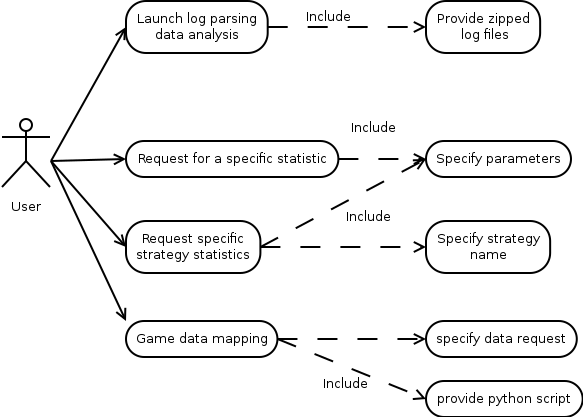
\includegraphics[scale=0.45,keepaspectratio]{UseCaseParsing}\\
Before the use of any features of the program , the user has to launch the parsing.
%L'interface utilisateur du programme sera composé d'un exécutable (minière de domination) qui sera exécuté avec certains paramètres pour exécuter l'action souhaitée. Le schéma ci-dessous représente les différentes interactions disponibles pour l'utilisateur:
%Avant l'utilisation de toutes les fonctionnalités du programme, l'utilisateur doit lancer l'analyse.
\subsection{Launching the log parsing}
%Lancement de l'analyse du journal
\subsubsection{Description and Priority}
%Description et priorité
\textbf{Priority level=high}\\
%Niveau de priorité = haute
\begin{itemize}
  \item The user will have to place all the compressed logs (tar.bz2 files) to be parsed into a
    specific folder.
  \item Once the previous step is done, the user can execute the parsing by
      typing : \textit{dominionmining parse (zlib/snappy)} if no compression is
      given the default compression is \textit{snappy}.
    \item For testing purposes, in order to avoid having a 4 hours parsing step, the user can specify a percentage of the logs to be parsed. by specifing a value between 0 and 100. the parser will randomly select logs from the provided ones and parse them, creating a usable database for further testing.
    \item once the parsing is done a message will be shown on the
      console (parsing done).
%L'utilisateur devra placer tous les journaux compressés (fichiers tar.bz2) pour être analysées dans un dossier spécifique.
%Une fois l'étape précédente est terminée, l'utilisateur peut exécuter l'analyse en tapant: dominion mining  analyse  (zlib / snappy) si aucune compression est donnée la compression par défaut est accrocheur.
%Pour des fins de test, afin d'éviter d'avoir un 4 heures étape d'analyse, l'utilisateur peut spécifier un pourcentage des journaux pour être analysée. en spécifiant une valeur comprise entre 0 et 100. l'analyseur choisira au hasard les journaux de ceux qui sont prévus et les analyser, en créant une base de données utilisable pour des tests supplémentaires.
%Une fois que l'analyse est effectuée un message sera affiché sur la console (traitement de fait).
\end{itemize}

\subsection{Statistics requests}
%Statistiques demandées
\subsubsection{Description and Priority}
%Description et priorité
\textbf{Priority level=high}\\
%Niveau de priorité = haute
The request for a statistic can be made by typing \textit{dominionmining stats (parameters)}.  \\
The possible strategy names are:
bigmoney , penprovince , beyondsilver.\\
If other strategies are recognized by the program they will be added to the list.\\
The list of parameters that will be possible to use will be determined in the
future.\\

The return of a statistic can be a chart displayed in a window or exported to a
file. If its a single value, a name or a sentence it will be returned in the prompt.
%La demande d'une statistique peut être faite en tapant les états de  dominion mining (paramètres).
%Les noms de stratégie possibles sont: big money, pen province, beyond silver.
%Si d'autres stratégies sont reconnues par le programme, ils seront ajoutés à la liste.
%La liste des paramètres qui seront possible d'utiliser sera déterminée dans le futur.
%Le retour d'une statistique peut être un graphique affiché dans une fenêtre ou exportés vers un fichier. Si sa une valeur unique, un nom ou une phrase, il sera retourné à l'invite.

\subsection{Game data mapping}
%Mappage des données de jeu
In order to allow the user to ask for specific statistics concerning a game, the program can be run in order to generate simplified game logs and then a python script will be applied to this log. This would allow more flexibility in the type of statistics displayable by the program.
%Afin de permettre à l'utilisateur de demander des statistiques spécifiques concernant un jeu, le programme peut être exécuté afin de générer des journaux de jeu simplifiées et un script python sera appliqué à ce journal. Cela permettrait une plus grande flexibilité dans le type de statistiques affichables par le programme.
\begin{itemize}
\item the program will be launched by using the following command: \textit{dominionmining data\_to\_query user\_script.py}
 \item the python script will be applied to the generated result and return the statistics asked by the user.
\item The generated file containing the query results will have the following format:
\begin{itemize}
\item The name of the produced file is \textit{game.txt}
\item The simplified log will contain each action made by the player, one action per line. List of actions and their format:
%Le programme sera lancé en utilisant la commande suivante: dominionmining data pour interroger l'utilisateur script.py
%Le script python sera appliquée au résultat généré et retourner les statistiques demandées par l'utilisateur.
%Le fichier généré contenant les résultats de la requête aura le format suivant:
%Le nom du fichier produit est game.txt
%Le journal simplifié contiendra chaque action effectuée par le joueur, une action par ligne. Liste des actions et leur format:
\begin{itemize}
\item Revealing a card: \textit{player\_x reveals card\_name}
\item Drawing cards: \textit{player\_x draws n cards}
\item Buying a card: \textit{player\_x buys card\_name}
\item Trashing cards: \textit{player\_x trashes n cards}
\item Puts a card: \textit{player\_x puts card\_name}
\item Gaining a card: \textit{player\_x gains card\_name}
\item Plays a card: \textit{player\_x plays card\_name}
%Révéler une carte: le joueur x révèle nom de la carte
%Piocher des cartes: le joueur x attire n cartes
%L'achat d'une carte: le joueur x achète nom de la carte
%Jeter des cartes : le joueur x jette n cartes
%Mettre une carte: le joueur x met le nom de la carte
%Le gain d'une carte: le joueur x joue le nom de la carte 
%Jouer une carte: le joueur x joue le nom de la carte
\end{itemize}
\end{itemize}
\end{itemize}

\section{Data Modeling}
%Modélisation des données

\subsection{Log decompression}
%Décompression des journaux
\subsubsection{Description and Priority}
%Description et priorité
\textbf{Priority level=high}\\

%Niveau de priorité = haute
\begin{itemize}
  \item The tar.bz2 files will be stored in a folder.
  \item The program will decompress one specified file from this folder in a temporary folder.
  \item The programm will delete the decompressed logs on demand by the parser.
%Les fichiers tar.bz2 seront stockés dans un dossier.
%Le programme va  décompresser un fichier spécifié à partir de ce dossier dans un dossier temporaire.
%Le programme va  supprimer les journaux décompressés  à la demande par l'analyseur.
\end{itemize}

\subsection{Parser}

\subsubsection{Description and Priority}
%Description et priorité
\textbf{Priority level=high}\\
%Niveau de priorité = haute
Provided the issues revealed by the logs (like: the inconsistency of the syntax)
a use of a parser made with tools like \textit{YACC and LEX} is not recommended.
For that a parser will be done by using the already present \textit{HTML} and
key words presents on the logs.\\
The parser is responsible for reading the logs and collecting the important
information without losing the structure of the log.\\
A glimpse of the data to be recognized by the parser is illustrated in this
diagram (some data to be determined as all the possibilities inside a log
haven't been revealed yet):\\

\includegraphics[scale=0.35,keepaspectratio]{UseCaseParser}
%À condition que les problèmes révélés par les journaux (comme: l'incohérence de la syntaxe) une utilisation d'un analyseur fait avec des outils comme YACC et Lex est déconseillée.
%Pour qu'un analyseur se fera en utilisant le déjà présent HTML et les mots clés présents sur les journaux.
%L'analyseur est chargé de lire les journaux et la collecte de l'information importante sans perdre la structure du journal.
%Un aperçu des données pour être reconnu par l'analyseur est illustré dans ce diagramme (certaines données à déterminer que toutes les possibilités de l'intérieur d'un journal n’ont pas encore été révélées):
\begin{itemize}
\item Winners: The list of the winners of the game, it can be one winner or several winners if they are tied.
\item Market: The list of 10 available cards to be bought by the players.
\item Cards Gone: list of cards that have been entirely bought at the end of the game.
\item Player Name: Name of the player.
\item Victory points: Amount of points at the end of the game.
\item Player cards: List of cards bought by the player with the amount they bought.
\item Victory cards: List of victory cards the player with the bought.
\item Trash: List of cards that that are discarded at the end of the game.
\item Game Moves: Every action depending on this item correspond to an action performed during a player's turn.
\end{itemize}
%Winners: La liste des gagnants du jeu, il peut être un gagnant ou plusieurs, les gagnants si elles sont liées.
%Market: La liste des 10 cartes disponibles pour être acheté par les joueurs.
%Cartes Gone: liste des cartes qui ont été entièrement acquises à la fin de la partie.
%Player Name: Nom du joueur.
%Victory points: nombre de points à la fin de la partie.
%Player cards: Liste des cartes achetées par le joueur avec le montant qu'ils ont acheté.
%Victory cards: Liste des cartes de victoire le joueur avec le acheté.
%Trash: Liste des cartes qui sont jetés à la fin de la partie.
%Game Moves: Chaque action en fonction de ce point correspond à une action effectuée pendant le tour d'un joueur.
The parser has to read every element shown in the previous graph as a part of the data when the user launches the parsing process.\\
%Le parser doit lire chaque élément montré dans le graphique précédent en tant que partie des données lorsque l'utilisateur lance le processus d'analyse.

\subsection{Create game-log}
%Créer game-log
\subsubsection{Description and Priority}
%Description et priorité
\textbf{Priority level=high}\\
%Niveau de priorité = haute
This functionality is the creation of a data structure where the log data will
be remodeled into.
here is a graphical representation of an overview of the data structure:\\
%Cette fonctionnalité est la création d'une structure de données où les données du journal seront rénovées.
%Voici est une représentation graphique d'une vue d'ensemble de la structure de données:
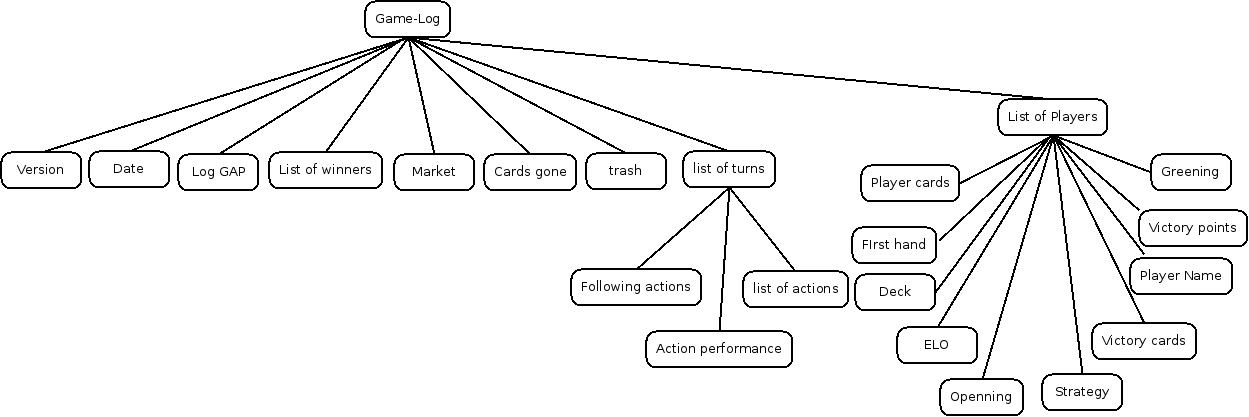
\includegraphics[scale=0.5,keepaspectratio]{game-log}

\subsection{Send game-log data}
%Envoyer des données de game-log
\subsubsection{Description and Priority}
%Description et priorité
\textbf{Priority level=high}\\
%Niveau de priorité = haute
The program will send the game-log data structure to the database part of the project.
%Le programme va envoyer la structure de données journal de jeu à la partie du projet de base de données.
\section{Data Storage}
%Stockage des données

\subsection{Connect to Relational Database}
%Se connecter à la base de données relationnelle
\subsubsection{Description and Priority}
%Description et priorité
\textbf{Priority level=high}\\
%Niveau de priorité = haute
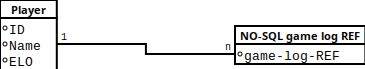
\includegraphics[keepaspectratio]{SQL}
\begin{itemize}
\item The program will be able to send data relative to the player (eg: ID, Name, Elo, Games played by the player)
\item The program will be able to send requests to the database concerning every piece of data stored in it.
\item The relational database will send the results of the requests made by the program.
%e programme sera capable d'envoyer des données reliées au joueur (par exemple: ID, Nom, Elo,  parties jouées par le joueur)
%Le programme sera capable d'envoyer des requêtes à la base de données relatives à chaque élément de données stockées.
%La base de données relationnelle va envoyer les résultats des demandes effectuées  par le programme.
\end{itemize}


\subsection{Create document-oriented Database}

\subsubsection{Description and Priority}
\textbf{Priority level=high}\\
This module will be responsible to create the document-oriented database containing data at the JSon format.
%Ce module sera responsable pour créer la base de données orientée document, contenant des données au format JSON.
\subsection{Connect to document-oriented Database}
%Se connecter à la base de données orientée document 
\subsubsection{Description and Priority}
%Description et priorité
\textbf{Priority level=high}\\
%Niveau de priorité = haute
\begin{itemize}
\item The document-oriented database will be handling exchanges through a specific socket.
\item The document-oriented database will receive game-logs at the JSon format.
\item The document-oriented database will receive requests from the program concerning every piece of data contained in it.
\item The document-oriented database will send results of the requests made by the program.
%La base de données orientée document sera en charge des échanges à travers un socket spécifique.
%La base de données orientée document recevra les journaux de jeu au format JSON.
%La base de données orientée document recevra les demandes du programme relatif à chaque élément de données qu'il contient.
%La base de données orientée document enverra les résultats des demandes effectuées par le programme.
\end{itemize}


\subsection{Compression}
\subsubsection{Description and Priority}
%Description et priorité
\textbf{Priority level=medium}\\
%Niveau de priorité = moyen
The document-oriented database will hold most of the data and some level of compression
will have to be applied.
The database in focus to be used at the moment is \textit{mongodb} and it offers
2 levels of compression \textit{Zlib} and \textit{Snappy}.
During the development the \textit{Snappy} will be used as it offers a better
performance.
But the final program should give the user the ability to chose the compression
level when starting the log parsing.
%La base de données orientée document contiendra la plupart des données et un certain niveau de compression devra être appliquée.
%La base de données qu’on va utiliser est focalisé pour le moment sur mongodb, et il offre 2 niveaux de compression Zlib et Snappy.
%Au cours du développement du Snappy sera utilisé car il offre une meilleure performance.
%Mais le programme final devrait donner à l'utilisateur la possibilité de choisir le niveau de compression lors du démarrage de l'analyse du journal.

\subsection{Save game-log}
%Sauvegarder la partie-journal
\subsubsection{Description and Priority}
%Description et priorité
\textbf{Priority level=high}\\
%Niveau de priorité = haute
\begin{itemize}
\item The document-oriented database will convert the game-log structure in a JSon formatted document.
\item The produced data in JSon format will be stored in the database.
%La base de données orientée document permet de convertir la structure journal de jeu dans un document au format JSON.
%Les données fournies au format JSON seront stockées dans la base de données.
\end{itemize}

\subsection{Load game-log}
%Chargement de game-log
\subsubsection{Description and Priority}
%Description et priorité
\textbf{Priority level=high}\\
%%Niveau de priorité = haute
When asked for a game-log, the database will load the JSon formatted log in a game-log data structure indetical to the one described in the data modelling section.\\
If there is missing information in the JSon document, the corresponding field will be left empty.
%Lorsque vous demandez un journal de jeu, la base de données va charger le journal au format JSON dans une structure de données de journal de jeu identique à celui décrit dans la section de la modélisation des données.
%S'il manque des informations dans le document JSON, le champ correspondant sera laissé vide.


\section{Data Analysis}
%Analyse des données 
\subsection{Gather data}
%Recueillir des données
\subsubsection{Description and Priority}
%Description et priorité
\textbf{Priority level=high}\\
%Niveau de priorité = haute
\begin{itemize}
\item The data analyser will convert the query results in a format usable by the plotting module.
\item If the data is simple to read (eg: a number, a name, a sentence), the data analyser will simply output the result in text format.
\item The last query will be memorized with it's result in order to gain time if the next query made by the user is the same.
\item If the user wants to apply a python script to game logs, the pogram will request the game logs and put them in a text file, this file will contain each action made by each player and the script will be applied to this file.
%L'analyseur de données va convertir les résultats de la requête dans un format utilisable par le module de traçage.
%Si les données sont simples à lire (par exemple: un numéro, un nom, une phrase), l'analyseur de données sera tout simplement envoyer le résultat au format texte.
%La dernière requête sera mémorisée avec son résultat afin de gagner du temps si la prochaine requête faite par l'utilisateur est le même.
%Si l'utilisateur souhaite appliquer un script python de journaux de jeu, le programme demandera les journaux de jeu et les mettre dans un fichier texte, ce fichier contiendra chaque action faite par chaque joueur et le script sera appliqué à ce fichier.
\end{itemize}

\subsection{restore game-log}
%Restaurer les game-log
\subsubsection{Description and Priority}
%Description et priorité
\textbf{Priority level=medium}\\
%%Niveau de priorité = moyen
This feature is responsible to restore the missing information on the parsed
logs, by using deduction based on the data obtained from the log.\\
In case of a missing game header or part of it missing:
%Cette fonction est responsable pour restaurer l'information manquante sur les journaux analysés, en utilisant la déduction basique sur la base des données obtenues par le journal.
%En cas d'un en-tête du jeu manquant ou partie manquante:
  \begin{itemize}
  \item Winners/victory cards/victory points missing: the program can keep track of the cards owned by the players during the game in order to know how many victory cards they have at the end of the game.
  \item Market missing: The program can keep track of the cards bought during the game in order to partially or totally reconstruct the cards available in the Market.
  \item Cards Gone: As with a missing Market data, the program will keep track of cards bought and count the amount bought for each card, if the maximum amount of cards is bought, the card is gone at the end of the game.
  \item Player name missing: the game moves part of a log also keeps track of the player names, the program will simply restore them in the header.
  \item Player cards: the program will keep track of the actions performed during the game relative to the player cards and add them in this list.
%Gagnants / cartes de victoire / points de victoire manquant: le programme peut garder la trace des cartes détenues par les joueurs pendant le jeu afin de savoir combien de cartes victoire qu'ils ont à la fin de la partie.
%Market manquant: Le programme peut garder la trace des cartes achetées au cours du jeu afin de reconstituer partiellement ou totalement les cartes disponibles sur Market.
%Cartes Gone: Comme avec les données manquantes de Market, le programme permet de garder une trace de cartes achetées et compter la quantité achetée pour chaque carte, si le montant maximum de cartes est acheté, la carte a disparu à la fin de la partie.
%Nom du joueur manquant: le jeu se déplace partie d'un journal assure également le suivi des noms des joueurs, le programme sera tout simplement de les restaurer dans l'en-tête.
%cartes de joueur: le programme permet de garder une trace des actions effectuées au cours du jeu par rapport aux cartes de joueurs et les ajouter dans cette liste.
  \end{itemize}

\subsection{Plotting}
\subsubsection{Description and Priority}
%%Description et priorité
\textbf{Priority level=high}\\
%Niveau de priorité = haute
The plotting module will get the converted data obtained after the Gather Data process and will plot them in a graphical interface. This module will work in a similar way of \textit{GnuPlot}.
%Le module de traçage va obtenir les données converties obtenues après le processus de recueillir des données et de les tracer dans une interface graphique. Ce module va fonctionner d'une manière similaire de GnuPlot.

\subsection{Calculate \textit{\textbf{ELO}}}
%Calculer ELO
\subsubsection{Description and Priority}
%Description et priorité
\textbf{Priority level=high}\\
%Niveau de priorité = haute
The analyzer will have to calculate the final ELO for each player and what was a
player ELO on a given game.
For each game in chronological order, this module will request the initial elo of the players from the relational database and the winners of the game, then it will calculate the new elo of each player from the outcome of the game. The module will then set the calculated elo in the document-oriented database at the currently analyzed game and will also update the overall elo for each of the players participating in the game on the relational database.\\
More information about ELO can be found on \url{https://en.wikipedia.org/wiki/Elo_rating_system}\\
The following diagram illustrates the process of the elo calculation:\\
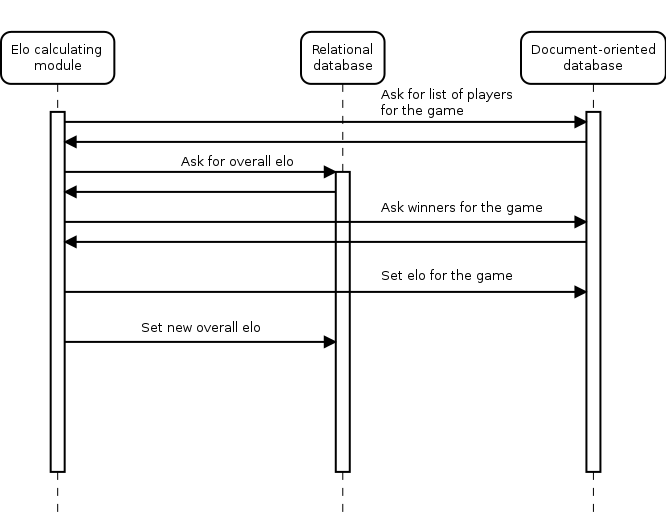
\includegraphics[width=\textwidth,height=\textheight,keepaspectratio]{elocalc}\\
%L'analyseur devra calculer la finale ELO pour chaque joueur et ce qui était un joueur ELO sur un jeu donné.
%Pour chaque jeu dans l'ordre chronologique, ce module va demander au elo initiale des joueurs de la base de données relationnelle et les gagnants du jeu, puis il va calculer la nouvelle elo de chaque joueur de l'issue du jeu.
%Le module sera ensuite définir le elo calculés dans la base de données orientée documents au jeu en cours d'analyse et mettra également à jour l'elo globale pour chacun des joueurs qui participent au jeu sur la base de données relationnelle.Plus d'informations sur ELO peuvent être consultés sur https://en.wikipedia.org/wiki/Elo_rating_system
%Le schéma suivant illustre le processus du calcul de elo:
\subsection{Recognize strategies}
%Reconnaître les stratégies
\subsubsection{Description and Priority}
%Description et priorité
\textbf{Priority level=medium}\\
%Niveau de priorité = moyen
The dominion wiki describes some strategies that can be used in the game .\\ For exemple :\\
Big Money\\
Beyond Silver \\
Penultimate Province Rule \\
More on \url{http://wiki.dominionstrategy.com/index.php/Strategy}\\

And the analyzer will have to be able to recognize what strategy was used on a
given match (if any strategy was used) and generate statistics.\\
\textbf{This image describes the decision process involved in the Big Money strategy}\\
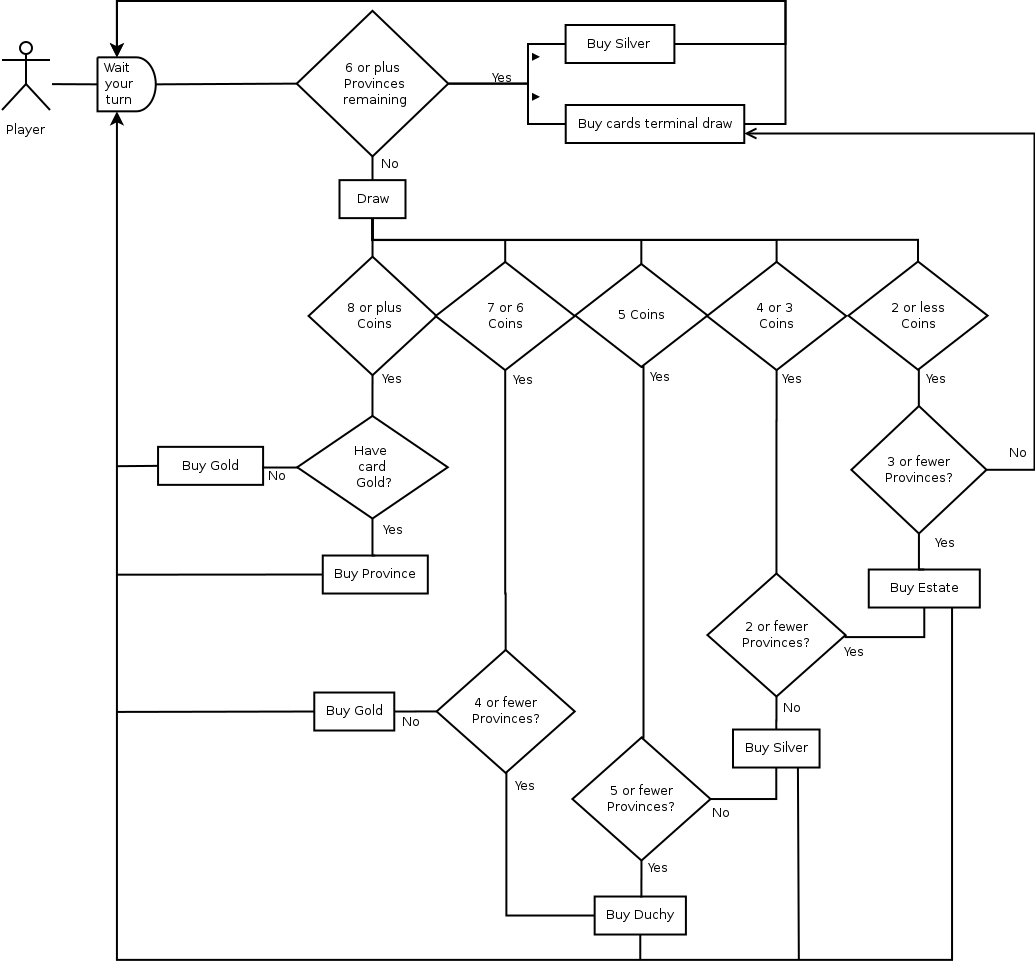
\includegraphics[width=\textwidth,height=\textheight,keepaspectratio]{big-money}\\
The analyzer has to recognize when a player buys only money cards and specific cards related to the big money strategy. It also has to keep track of the remaining provinces to be bought.\\
More on \url{http://wiki.dominionstrategy.com/index.php/Big_Money}\\
%Le wiki de domination décrit quelques stratégies qui peuvent être utilisés dans le jeu.

%Par exemple :
%Big Money
%Beyond Silver
%Penultimate Province Rule
%Plus de détails sur http://wiki.dominionstrategy.com/index.php/Strategy
%Et l'analyseur devra être en mesure de reconnaître quelle stratégie a été utilisée sur un match donné (si une  stratégie a été utilisée) et générer des statistiques.
%Cette image décrit le processus de décision associé à la stratégie Big Money

In order to recognize the strategy coined Beyond Silver, the analyzer has to recognize when certain type of cards are bought, the list of these cards can be found on. \url{http://wiki.dominionstrategy.com/index.php/Silver#Beyond_Silver}\\

In order to recognize that the Penultimate Province Rule is respected (as explained on \url{http://dominionstrategy.com/2011/03/28/the-penultimate-province-rule/}), the analyzer has to keep track of the amount of Victory Points of each player at every turn.
%Plus de détails sur http://wiki.dominionstrategy.com/index.php/Big_Money
%Afin de reconnaître la stratégie inventé Beyond Silver, l'analyseur doit reconnaître lorsque certains types de cartes sont achetés, la liste de ces cartes peuvent être trouvés sur : http://wiki.dominionstrategy.com/index.php/Silver#Beyond_Silver
%Afin de reconnaître que Penultimate Province Rule est respecté (comme expliqué à la http://dominionstrategy.com/2011/03/28/the-penultimate-province-rule/), l’analyseur doit garder une trace de la quantité de Points de Victoire de chaque joueur à chaque tour.
\subsection{Recognize Greening}
% Reconnaître Greening
\subsubsection{Description and Priority}
%Description et priorité
\textbf{Priority level=high}\\
%Niveau de priorité = haute
The analyzer has to be capable of recognize the \textit{\textbf{greening}} moment on each match.
More about \textit{\textbf{greening}} on \url{http://wiki.dominionstrategy.com/index.php/Greening}.\\
The program will recognize when the greening happens by detecting when victory cards begin to be bought.
%L'analyseur doit être capable de reconnaître le moment de Greening sur chaque match. En savoir plus sur l'écologisation sur http://wiki.dominionstrategy.com/index.php/Greening.
%Le programme reconnaître quand greening arrive en détectant lorsque les cartes de victoire commencent à être achetées.

\chapter{Nonfunctional Requirements}
%Besoins non fonctionnels
\section{Performance Requirements}
%Besoins de performance
% $<$If there are performance requirements for the product under various
% circumstances, state them here and explain their rationale, to help the
% developers understand the intent and make suitable design choices. Specify the
% timing relationships for real time systems. Make such requirements as specific
% as possible. You may need to state performance requirements for individual
% functional requirements or features.$>$
No specific performance requirement was made by the client. But for the analyzer
a time of running should be less than an hour.\\
The user should be able to iterate the analysis process on a precise dataset without having to wait for the same query to be done again.
%Aucun besoin de performance spécifique n’a été faite par le client. Mais pour l'analyseur le temps d’exécution  doit être inférieur à une heure.
%L'utilisateur doit être capable de parcourir le processus d'analyse sur un ensemble de données précis sans devoir attendre que la même requête à refaire.


\section{Reliability}
% Fiabilité
The client demands that the maximum number of logs should be parsed , as the
data provided has some inconsistencies and some logs wont be possible to parse.
the client agrees that between 5 to 10\% of the logs can be ignored.\\

The parser will have to parse 100\% of the data present on the log and Restore
any missing information if possible.\\
%Le client demande que le nombre maximum de journaux doivent être analysé, que les données fournies ont des incohérences et quelques journaux ne seront pas possibles d'analyser.
%L'analyseur devra analyser 100% des données présentes sur le journal et restaure toute information manquante si possible.
\section{Software Quality Attributes}
%Attributs de qualité de logiciels
% $<$Specify any additional quality characteristics for the product that will be
% important to either the customers or the developers. Some to consider are:
% adaptability, availability, correctness, flexibility, interoperability,
% maintainability, portability, reliability, reusability, robustness, testability,
% and usability. Write these to be specific, quantitative, and verifiable when
% possible. At the least, clarify the relative preferences for various attributes,
% such as ease of use over ease of learning.$>$
Even if just a command line is expected for the final program it should have a
easy learn curve and be easy to use.\\
The data generated by the parser don't need to be human readable.\\
The game logs generated will have to be analyzeable by the user in order to allow as much flexiblity as possible in the treatment of the logs.
%Même si seulement une ligne de commande est prévue pour le programme final, elle devrait avoir une courbe facile à apprendre et être facile à utiliser.
%Les données générées par l'analyseur n’ont pas besoin à être lisible par l'homme.
%Les journaux de jeux générés devront être analysés par l'utilisateur afin de permettre la plus grande souplesse possible dans le traitement des journaux.

%\chapter{Other Requirements}
% $<$Define any other requirements not covered elsewhere in the SRS. This might
% include database requirements, internationalization requirements, legal
% requirements, reuse objectives for the project, and so on. Add any new sections
% that are pertinent to the project.$>$

%\section{Appendix A: Glossary}
% %see https://en.wikibooks.org/wiki/LaTeX/Glossary
% $<$Define all the terms necessary to properly interpret the SRS, including
% acronyms and abbreviations. You may wish to build a separate glossary that spans
% multiple projects or the entire organization, and just include terms specific to
% a single project in each SRS.$>$

%\section{Appendix B: Analysis Models}
% $<$Optionally, include any pertinent analysis models, such as data flow
% diagrams, class diagrams, state-transition diagrams, or entity-relationship
% diagrams.$>$

%\section{Appendix C: To Be Determined List}
% $<$Collect a numbered list of the TBD (to be determined) references that remain
% in the SRS so they can be tracked to closure.$>$

\end{document}
